% s1_aft cut, because I apparently need to include this

\chapter{APPENDIX B}\label{app:s1aft} % because apparenlty 'Data selection using s1_area_fraction_top' isn't acceptable. GFY grad school

\paragraph{Abstract} While a detector like XENON1T records several events every second, a significant fraction of these are not of interest to most analyses. Data selection criteria must be developed to filter good events from the unwanted. In this chapter we describe the development of a simple cut using the \textit{area\_fraction\_top} property of an interaction's S1 peak. This cut was used for the analysis of both SR0~\cite{Aprile:2017iyp} and SR1 (publication in preparation).

\section{Introduction}

For each S1 and S2 peak recorded in the XENON1T detector, a wide variety of properties are computed. One of these is the \textit{area\_fraction\_top}, which is the fraction of the peak's area measured by the top PMT array (sometimes called `asymmetry' in similar experiments). While this quantity is largely constant for all S2 peaks (due to the tightly-constrained space in \textit{z} where the S2s are generated), for S1 peaks this quantity can change significantly. This can be used as a verification for the reconstructed \textit{z} coordinate of the interaction (based on the drift time) by comparing the measured \textit{s1\_area\_fraction\_top} to the expected value, given the reconstructed location vertex.

\section{\textit{area\_fraction\_top} throughout the detector}

First we must determine, for all positions in the detector, what the probability is that a photon created will be observed by the top array (the \textit{area\_fraction\_top} quantity). While this is entirely geometrically determined, factors such as reflection from the walls and total internal reflection off the liquid surface mean it is easier to determine this relationship from data rather than from a Monte Carlo simulation or a closed-form expression. The $32\1{keV}$ line from $^{83m}$Kr is well-suited for this measurement, as about 250 photons are detected from this peak. This is a large enough number to suppress statistical fluctuations from very low-energy signals, but not so large that PMT saturation becomes important.

\subsection{Event selection}

Events are selected from the XENON1T SR1 $^{83m}$Kr calibration data. We require events with two S1s, the first between 210 and 300 PE, the second between 63 and 113 PE, as shown in Figure~\ref{fig:s1a_s1b}. Further, we require that the interactions with both S1s are reconstructed in the same location. As the requirements for these events are not very tight, the tolerance on the selection requirements are quite loose.

\begin{figure}[htb]
    \centering
    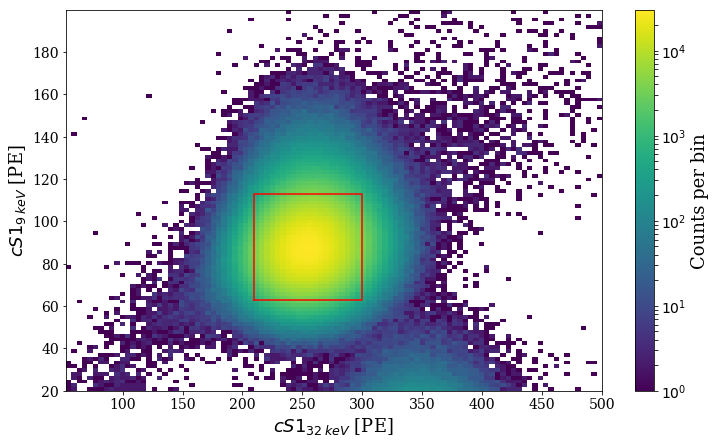
\includegraphics[width=0.8\textwidth]{figures/s1aft/sr1_83mkr_s1s}
    \caption{The double-decay structure of $^{83m}$Kr makes selection of events with resolved S1s very straightforward. Events within the box are selected, giving a total of 5.8~million events.}\label{fig:s1a_s1b}
\end{figure}

We will focus on the $32\1{keV}$ line, which is the first and larger of the S1s. The relationship between $z$ and \textit{s1\_area\_fraction\_top} of this population is shown in Figure~\ref{fig:z_aft}. Events near the cathode have \textit{s1\_area\_fraction\_top} around 0.09, while events near the gate have \textit{s1\_area\_fraction\_top} around 0.38.

\begin{figure}[htb]
\centering
    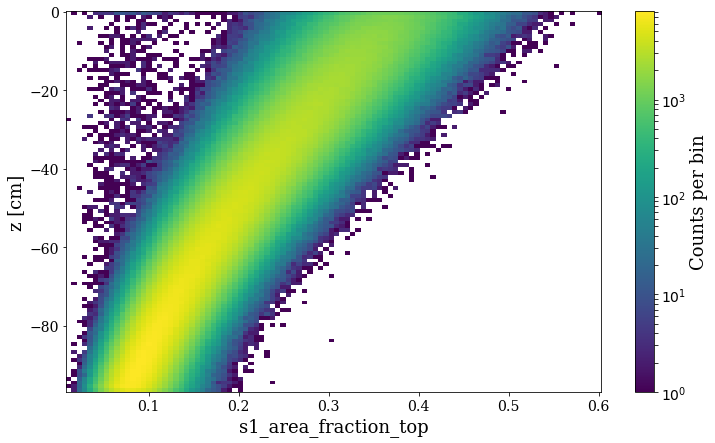
\includegraphics[width=0.8\textwidth]{figures/s1aft/z_s1aft}
    \caption{\textit{s1\_area\_fraction\_top} depends strongly on $z$, shown here using events from the $32\1{keV}$ line from $^{83m}$Kr.}\label{fig:z_aft}
\end{figure}

\subsection{area\_fraction\_top map}

While \textit{s1\_area\_fraction\_top} depends most strongly on $z$, we also investigate any radial dependence. To do this we bin the detector into 476~bins by making selections in $z$, $r$, and $\phi$, exploiting the cylindrical symmetry of the active region. As we expect the strongest radial dependence to be in the regions closest to the PMT arrays and the edges of the detector, we employ variable bin widths in $z$, with bins at the ends of the detector being $4\1{cm}$ wide, increasing to $9\1{cm}$ in the center. Bins are uniformly spaced in $r^2$, and are divided into 4~wedges in the center, increasing to 12~wedges near the edges of the detector. For events in each bin, we take the median value of \textit{s1\_area\_fraction\_top}. We show the results in Figure~\ref{fig:s1_aft_map}. Radial variations are minimal except for the top few centimeters near regions where several PMTs are nonfunctional, and the bottom few centimeters near the circumference of the detector.

\begin{figure}[htpb]
\centering
    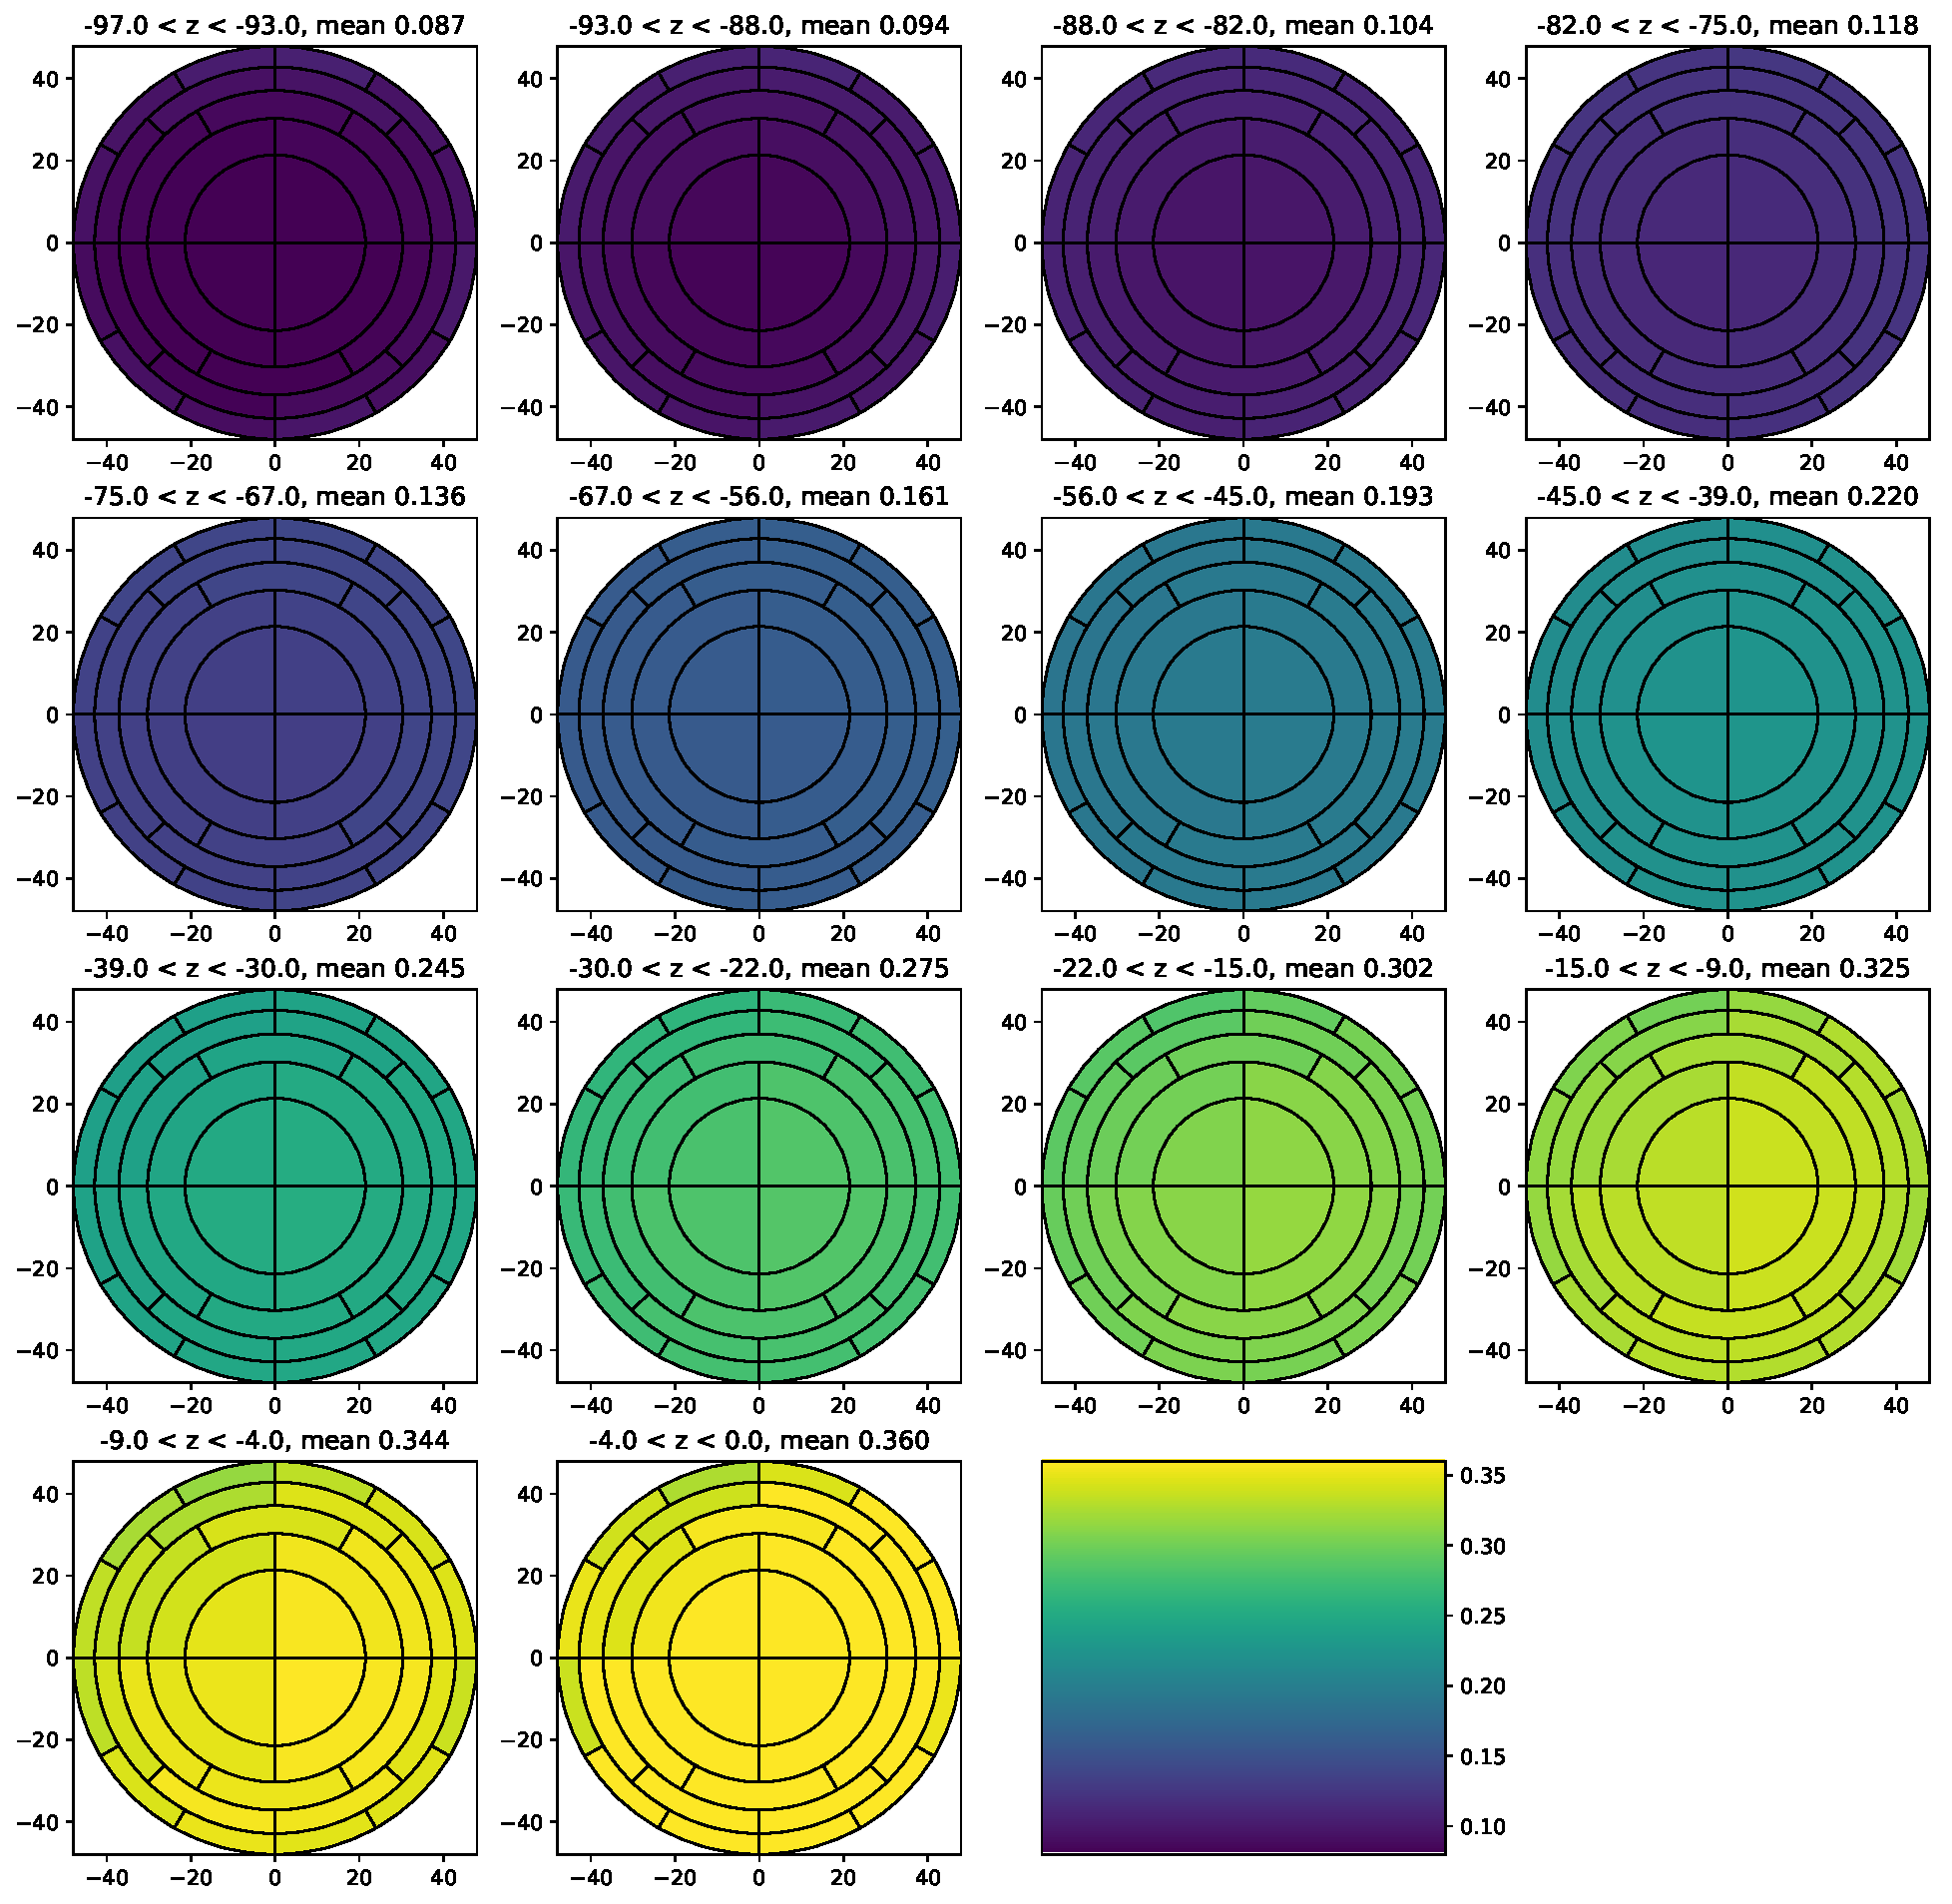
\includegraphics[width=\textwidth]{figures/s1aft/s1aft_binned_44}
    \caption{\textit{s1\_area\_fraction\_top} throughout the XENON1T detector, measured using events from the $32\1{keV}$ line of $^{83m}$Kr. While the $z$ dependence dominates, a small radial component also is visible near the ends of the detector.}\label{fig:s1_aft_map}
\end{figure}

\section{S1AreaFractionTop Cut}

The map of \textit{s1\_area\_fraction\_top} gives us the probability that a photon created at a given location in the detector reaches the top PMT array. As photons are created independently from each other, the number photons reaching the top PMT array will be binomially distributed. This allows us to calculate a p-value for an interaction by comparing the number of photons measured by the top PMT array to the expected number of photons, given the reconstructed position of the interaction. We use the \texttt{binom\_test} routine from the \texttt{stats} module in the \texttt{scipy} Python package, with an extension to accomodate floating-point inputs rather than integers (primarily using the gamma function rather than the factorial function). We show the overall behavior of the p-value in Figure~\ref{fig:z_aft_pval}. As shown, events near the center of the band have higher p-values than events further from the center.

\begin{figure}[htb]
\centering
    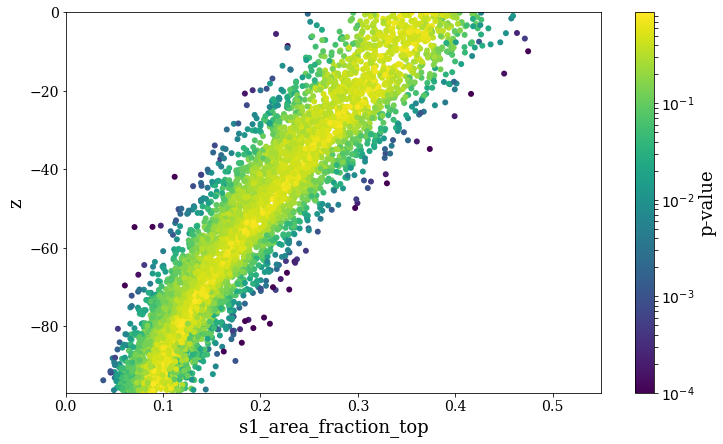
\includegraphics[width=\textwidth]{figures/s1aft/z_aft_pval}
    \caption{P-value distribution in the parameter space favorable for visualization. Events further from the center of the band have progressively smaller p-values.}\label{fig:z_aft_pval}
\end{figure}

We can set a minimum p-value for ``good'' events at $1\times10^{-3}$ to reject events leaking below the nuclear recoil band. We evaluate the acceptance of this cut to simulated data using the Wilson confidence interval for events both within and without the fiducial volume, as shown in Figure~\ref{fig:accept}. The acceptance is $>95\%$ within the fiducial volume for the dark matter signal region. The slight dip around 5~PE is due to a simulation artifact and is not seen in data.

\begin{figure}[htb]
\centering
    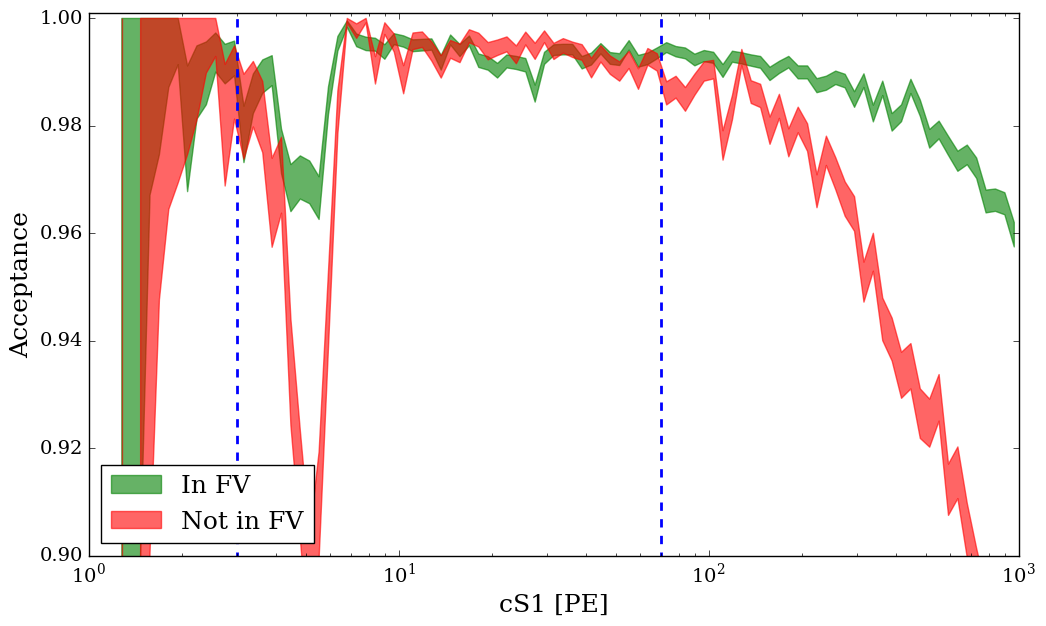
\includegraphics[width=\textwidth]{figures/s1aft/s1aftacceptance}
    \caption{Acceptance for the S1AreaFractionTop cut for a minimum p-value of $1\times10^{-3}$, calculated using the Wilson confidence interval on simulated data. The vertical blue lines are the bounds on the dark matter signal region. Within the fiducial volume the acceptance is high, and the acceptance only decreases well beyond the signal region. The dip around 5~PE is due to an artifact in the waveform simulator where it assumes a slightly different relationship between $z$ and \textit{s1\_area\_fraction\_top} than shown in Figures~\ref{fig:z_aft} and~\ref{fig:z_aft_pval}. On real data this dip is not seen.}\label{fig:accept}
\end{figure}

As this cut is based on a p-value, tuning its performance is very easy. If combined with other p-value-based cuts, additional cutting power can be gained in edge cases.
